
\section{\fontsize{14}{0}\selectfont Realice un proceso completo de análisis usando pipeline}
\subsection{ Descripción del Dataset}
Para el caso de estudio usando Pipeline, se hizo uso del dataset Haberman, del siguiente enlace \url{https://archive.ics.uci.edu/ml/datasets/Haberman\%27s+Survival}, el cual describe, sobre la evolución y supervivencia de mujeres que hayan sido operadas, para tratar el cáncer de mama, las columnas del dataset son los siguientes: 
\begin{itemize}
	\item Edad: Edad de las mujeres, cuando fueron sometidas a la operación. 
	\item Año de intervención quirúrgica: restando 2000-1900, la columna muestra el año en el que se realizaron la operación. 
	\item Ganglios: Es un número entero, el cual nos señala, cuantos ganglios cancerosos fueron detectados.
	\item Supervivencia: 1 si sobrevivió más de 5 años después de la operación, 2 si murió entre los 5 años.  
\end{itemize}
Para resolver el problema, se efectuó los siguientes procedimientos 
\begin{itemize}
	\item El dataset fue divido en X\_train y Y\_train, donde el primero representa a la edad, año de operación y ganglios cancerosos, el segundo hace referencia a la supervivencia de las mujeres.
	\item Ambas matrices la primera matriz fue normalizada y estandarizada, posterior a esto se volvió a fraccionar en la matriz de entrenamiento y la de prueba, donde el porcentaje es 80 y 20.
	\item Las pruebas fueron realizadas usando pipeline en conjunto con la regresión logística y una prueba singular con la regresión logística, esto con el objetivo de comparar los resultados.

	
\end{itemize}
Todo el análisis anterior, está desarrollado bajo el siguiente código:

\begin{lstlisting}[language=python]
import numpy as np
import pandas as pd
from sklearn import preprocessing as pre
from sklearn import linear_model as lm
from sklearn.preprocessing import Normalizer as nm
from sklearn.preprocessing import StandardScaler as sc
from sklearn.model_selection import train_test_split
from sklearn.preprocessing import StandardScaler
from sklearn.pipeline import Pipeline
from sklearn.svm import SVC
from sklearn.linear_model import LogisticRegression

# cargamos el dataset
dato = pd.read_csv("haberman.csv")

aux = np.array(dato[['edad', 'year', 'auxilia']])
norm = nm().fit(X=aux).fit_transform(X=aux)
standar = sc().fit(X=norm).fit_transform(X=norm)
aux2 = np.array(dato[['supervivencia']])
norm2 = nm().fit(X=aux2).fit_transform(X=aux2)
X_train, X_test, y_train, y_test = train_test_split(standar,
aux2,
test_size=0.2,
random_state=0
)
pipe = Pipeline([('scaler', StandardScaler()),
('svc', LogisticRegression(random_state=42))])
doge = lm.LogisticRegression(random_state=42)
doge.fit(X_train, y_train)
print("Resultados obtenidos con la regresión logistica ",
doge.score(X_test, y_test))
print("Predición de esperanza de vida de una mujer con cancer usando pipeline
, bajo las siguientes caracteristicas\nedad=30\nAño de Operación = 1960 ",
"Ganglios cancerosos encontrados = 23 \nResultado = ", doge.predict([[30, 60, 23]]))
pipe.fit(X_train, y_train)
print("Resultados obtenidos con la regresión logistica usando pipeline",
pipe.score(X_test, y_test))
print("Predición de esperanza de vida de una mujer con cancer usando pipeline,
 bajo las siguientes caracteristicas\nedad=30\nAño de Operación = 1960 ",
"Ganglios cancerosos encontrados = 23 \nResultado = ", pipe.predict([[30, 60, 23]]))
\end{lstlisting}
De donde se obtiene los siguientes resultados:
\begin{figure}[H]
	\centering
	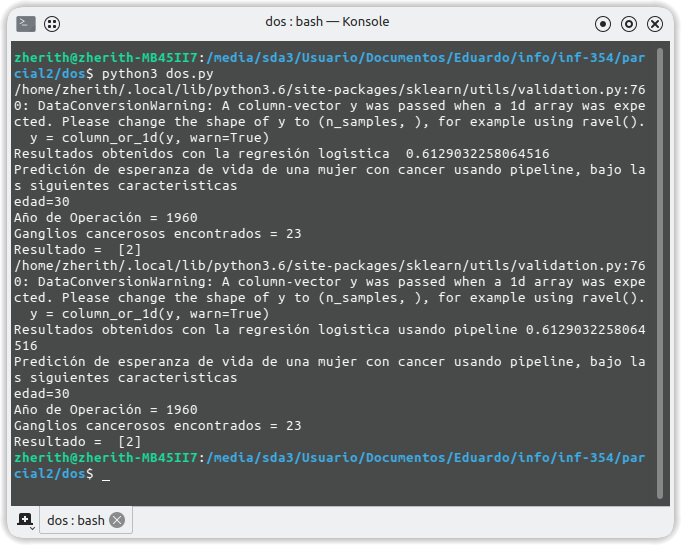
\includegraphics[width=0.8\linewidth]{im/uno.png}
	\caption[Resultados Obtenidos del Dataset Haberman, usando Pipeline]{Resultados Obtenidos del Dataset Haberman,usando Pipeline}
\end{figure}
Se puede ver que en ambos casos se obtuvo un resultado cerca de 0.61, y una predicción correcta. 






